\subsection{Pearson Correlation}\label{subsec:pearsoncorrelation}

Drive-LaB will score trips based on the scoringmodel described in Section \ref{subsec:prereq}. The scoringmodel is based on six metrics, roadtypes, critical time periods, speeding, accelerations, brakes and jerks, decided upon in \citep{sw9_report}. These six metrics cover a big part of the drivers performance during a trip, but it is essential to verify the importance of each individual metric when identifying driver style. Such an experiment can be conducted by computing a Pearson correlation matrix, in order to ensure that no metrics are directly correlating, meaning one of the metrics is negligible. This experiment is run in coherence with the chosen policy, as described in Section \ref{subsec:policy}. The Pearson correlation is calculated on the scores of the metrics on the given trips.

The matrix of Pearson correlations between the metrics is shown in Table \ref{tab:pearsonmatrix}. The most notable result is the multicollinearity between accelerations and brakes, which seems rather odd as they are diametrical opposites and can per definition not exist at the same time. Another highly correlating metric is jerks, having a correlation of 0.828 with both brakes and accelerations. 

\begin{table*}[tb]
\centering
\caption{This is the Pearson correlation matrix between the metrics}
\label{tab:pearsonmatrix}
\begin{tabular}{|l|llllll|}
\hline
\rowcolor{tablegreen}
                      & \textbf{Roadtypes} & \textbf{Critical Time Periods} & \textbf{Speeding} & \textbf{Accelerations} & \textbf{Brakes} & \textbf{Jerks} \\\hline
Roadtypes             & 1 &  &  &  &  &  \\
Critical Time Periods & -0.250    & 1  &  &  &  &  \\
Speeding              & -0,546    & 0.156                 & 1  &  &  &  \\
Accelerations         & -0.341    & 0.460                 & 0.196    & 1  &  &   \\
Brakes                & -0,348    & 0.428                 & 0.195    & 0.971         & 1 &   \\
Jerks                 & -0,241    & 0.313                 & 0.144    & 0.828         & 0.828  & 1 \\\hline  
\end{tabular}
\end{table*}

Looking closer at the multicollinearity between accelerations and brakes, there are a couple of different factors which affect the result. As mentioned, accelerating and braking are diametrically opposite, but they are both dependent on the speed of the vehicle (as they are calculated through the change in speed). Given a trip starts and ends at the same speed(0 km/t), the accumulated acceleration must be equal to the accumulated brake.

\begin{figure}[tb]
\centering
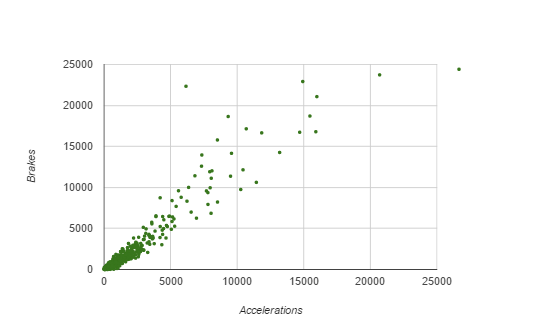
\includegraphics[width=0.465\textwidth]{Pictures/abcorrel}
\caption{A scatterplot of the correlation between acceleration- and brake score}
\label{fig:abcorrel}
\end{figure}

Figure \ref{fig:abcorrel} clearly illustrates the correlation between accelerations and brakes. Another reason as to why these metrics correlate can be the thresholds in the policy used to calculate the scores. As earlier mentioned the threshold for brakes are 8 $m/s^2$ whereas accelerations are counted from 5 $m/s^2$. If we had no thresholds and the delinquencies were scored the same, the correlation would be 1.0 as it only depended on the speed of the vehicle. 
Jerks was the metric that met the highest level of skepticism when the scoringmodel was designed, and the correlation shows that it was not completely unwarranted. It does show a lot of correlation with both brakes and accelerations. Figure \ref{fig:ajcorrel} shows the correlation between accelerations and jerks. Jerks are, as mentioned, calculated as $m/s^3$, and a driver with many accelerations are almost bound to have a lot of jerks as it is hard to keep a constant acceleration.

\begin{figure}[tb]
\centering
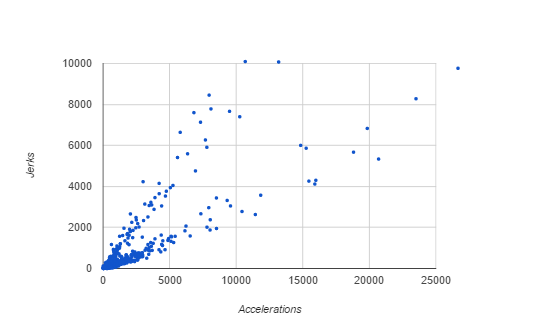
\includegraphics[width=0.465\textwidth]{Pictures/ajcorrel}
\caption{The correlation between acceleration- and jerkscore}
\label{fig:ajcorrel}
\end{figure}